\documentclass{article}
%
\usepackage{color}
\usepackage{mathtools}
% inclusão de figuras em PDF, PNG, PS, EPS
\usepackage{graphicx}
\usepackage{float}
\usepackage[export]{adjustbox}
\usepackage{bookmark}

% auto referencia
\usepackage{hyperref}
\hypersetup{
	%	hidelinks=true,
	colorlinks=true,
	linkcolor=blue,
	citecolor=blue,   
	urlcolor=blue,
}


\setlength\parindent{0pt}
\newcommand{\mdp}[2]{\frac{\partial #1}{\partial #2}}
\newcommand{\mdpv}[2]{\frac{\partial^2 #1}{\partial #2^2}}
\newcommand{\mdph}[3]{\frac{\partial^2 #1}{\partial #2 \partial #3}}
%---------------------------------------------------------------------------

\renewcommand*\contentsname{Índices}

\begin{document}
	
% -------------------------------------------------------------------------- 
\tableofcontents
% -------------------------------------------------------------------------- 

%---------------------------------------------------------------------------
\section{Formulação variacional}
%
Para considerando a equação diferencial:
%
\begin{equation}
	 \frac{d^2u}{dx^2} + f(x) = 0
	 \label{eq1:eq_dif}
\end{equation}
%
A formulação variacional pode-se ser obtida multiplicado e integrando a eq. (\ref{eq1:eq_dif}) em todo o domínio $L$.
%
\begin{equation}
	\int_0^L\left( \frac{d^2u}{dx^2} + f(x) \right) w(x) dx = 0
\end{equation}
%
Usando a regra da soma de integrais temos,
%
\begin{equation}
	\int_0^L \frac{d^2u}{dx^2} w(x) dx + \int_0^L f(x) w(x) dx= 0
\end{equation}
%
Focando apenas no primeiro termo,
%
\begin{equation}
	\int_0^L \frac{d^2u}{dx^2} w(x) dx  = \frac{du}{dx} w(x) \mid_0^L - \int_0^L \frac{du}{dx} \frac{dw}{dx} dx 
	\label{eq1:integral_por_partes}
\end{equation}
%
O que leva à,

\begin{equation}
	\frac{du}{dx} w \mid_0^L - \int_0^L \frac{du}{dx} \frac{dw}{dx} dx  + \int_0^L f(x) w(x) dx= 0
\end{equation}
%
\subsection{Integral por partes}
%
Para chegar na eq. (\ref{eq1:integral_por_partes}) considere primeiro a regra do produto parada derivas para duas funções genéricas $a(x)$ e $b(x)$:
%
\begin{equation}
	\frac{d(ab)}{dx} = \frac{da}{dx} b + \frac{db}{dx} a
\end{equation}
%
Integrando em ambos os lados,
%
\begin{equation}
	\int_0^L \frac{d(ab)}{dx} dx = \int_0^L \frac{da}{dx} b dx + \int_0^L \frac{db}{dx} a dx
\end{equation}
%
A integral e a deriva se cancelam no primeiro termo,
%
\begin{equation}
	ab|_0^L = \int_0^L \frac{da}{dx} b dx + \int_0^L \frac{db}{dx} a dx
\end{equation}
%
Considerando agora que $a(x) = \frac{du}{dx}$ e $b(x) = w(x)$, portanto 
%
\begin{equation}
	\frac{du}{dx} w|_0^L = \int_0^L \frac{d^2u}{dx^2} w dx + \int_0^L \frac{dw}{dx} \frac{du}{dx} dx
	\label{eq1:formu_var}
\end{equation}
%
levando assim  a eq (\ref{eq1:integral_por_partes}).
%
\subsection{Resíduos ponderados}
%
A aproximando $u(x)$ por $\hat u(x)$ eq. (\ref{eq1:eq_dif}) não e mais resolvida de maneira exata sobrenado um resíduo $R(x)$,
%
\begin{equation}
	\frac{d^2 \hat u}{dx^2} + f(x) = R(x)
\end{equation}
%
A ideia é reduzir este resíduo usando uma aproximação da função peso $\hat w(x)$.
%
\begin{equation}
	\int_0^L R(x) \hat w(x) dx=  \int_0^L\left( \frac{d^2\hat u}{dx^2} + f(x) \right) \hat w(x) dx = 0
\end{equation}
%
Os métodos do Elementos Finitos, Diferença Finita e Volume Finitos são gerados pelas diferentes escolhas das funções $w$. Usando a formulação variacional eq. \ref{eq1:formu_var} temos,
%
\begin{equation}
	\int_0^L \frac{d \hat u}{dx} \frac{d \hat w}{dx} dx  =  	\frac{d \hat u}{dx} \hat w \mid_0^L + \int_0^L f(x) \hat w(x) dx
	\label{eq1:Residuo_ponderados}
\end{equation}
%
\subsection{Aproximações}
%
As aproximações de $\hat u(x)$ e $\hat w(x)$ são dada por,
%
\begin{align}
	&\hat u(x) = \sum_{j = 1}^n N_j(x) u_j\\
	&\hat w(x) = \sum_{i = 1}^n N_i(x) w_i
\end{align}
%
onde $n$ é o número de pontos na malha. Substituindo $\hat w(x)$ na eq. (\ref{eq1:Residuo_ponderados})
%
\begin{equation}
\begin{split}
	\int_0^L \frac{d \hat u}{dx} \frac{d}{dx} \left(\sum_{i = 1}^n N_i(x) w_i\right) dx = \frac{d \hat u}{dx} \left(\sum_{i = 1}^n N_i(x) w_i\right) \mid_0^L  \\ + \int_0^L f(x)\left(\sum_{i = 1}^n N_i(x) w_i\right) dx
\end{split}
\end{equation}
%
Para o primeiro termo temos,
%
\begin{equation}
\begin{split}
	\int_0^L \frac{d \hat u}{dx} \frac{d}{dx} \left(\sum_{i = 1}^n N_i(x) w_i\right) dx =	\int_0^L \frac{d \hat u}{dx}  \frac{d}{dx} \left( N_1 w_1 + ... + N_n w_n \right) dx\\
	=\int_0^L \frac{d \hat u}{dx}  \left( \frac{dN_1}{dx} w_1 + ... + \frac{dN_n}{dx} w_n \right) dx\\
	=\int_0^L \frac{d \hat u}{dx}  \frac{dN_1}{dx} w_1 dx + ... + \int_0^L \frac{d \hat u}{dx}  \frac{dN_n}{dx} w_n dx\\
	=w_1 \int_0^L \frac{d \hat u}{dx}  \frac{dN_1}{dx} dx + ... + w_n \int_0^L \frac{d \hat u}{dx}  \frac{dN_n}{dx}  dx
\end{split}
\label{eq1:p_termo}
\end{equation}
%
Para o segundo termo temos,
%
\begin{equation}
	\begin{split}
	\frac{d \hat u}{dx} \left(\sum_{i = 1}^n N_i(x) w_i\right) \mid_0^L = w_1  \frac{d \hat u}{dx} N_1(x) \mid_0^L + ... + w_n \frac{d \hat u}{dx} N_n(x) \mid_0^L
	\end{split}
\label{eq1:s_termo}
\end{equation}
%
Para o terceiro termo temos,
%
\begin{equation}
	\begin{split}
		\int_0^L f(x)\left(\sum_{i = 1}^n N_i(x) w_i\right) dx = \int_0^L f(x)\left(N_1(x) u_1 + ... + N_n(x) w_n\right) dx\\
		= w_1 \int_0^L f(x) N_1(x) dx + ... + w_n \int_0^L f(x) N_n(x) dx
	\end{split}
\label{eq1:t_termo}
\end{equation}
%
%---------------------------------------------------------------------------
%
Juntando as eqs. (\ref{eq1:p_termo}), (\ref{eq1:s_termo}) e (\ref{eq1:t_termo}) temos,
%
\begin{equation}
	\begin{split}
    w_1 \int_0^L \frac{d \hat u}{dx}  \frac{dN_1}{dx} dx + ... + w_n \int_0^L \frac{d \hat u}{dx}  \frac{dN_n}{dx}  dx =\\
    w_1  \frac{d \hat u}{dx} N_1(x) \mid_0^L + ... + w_n \frac{d \hat u}{dx} N_n(x) \mid_0^L \\
    + w_1 \int_0^L f(x) N_1(x) dx + ... + w_n \int_0^L f(x) N_n(x) dx
	\end{split}
\end{equation}
%
Isolando agora os $w_i$,

\begin{equation}
	\begin{split}
		&w_1 \left(\int_0^L \frac{d \hat u}{dx}  \frac{dN_1}{dx} dx -  \frac{d \hat u}{dx} N_1(x) \mid_0^L -\int_0^L f(x) N_1(x) dx \right)\\
		&+ ... + \\
		&w_n \left(\int_0^L \frac{d \hat u}{dx}  \frac{dN_n}{dx} dx -  \frac{d \hat u}{dx} N_n(x) \mid_0^L -\int_0^L f(x) N_n(x) dx \right) = 0
	\end{split}
	\label{eq1:somatorio_i}
\end{equation}
%
Para que a eq (\ref{eq1:somatorio_i}) seja sempre verdade ou os $w_i$ são todos nulos ou as expressões são nulas. Fazer todos $w_i$ nulos não tem utilidade, logo a melhor opção é fazer todas as expressões dentro dos parenteses nulas. Assim nos temos um conjunto $n$ equações,
%
\begin{equation}
	\begin{split}
		&\int_0^L \frac{d \hat u}{dx}  \frac{dN_1}{dx} dx -  \frac{d \hat u}{dx} N_1(x) \mid_0^L -\int_0^L f(x) N_1(x) dx  = 0\\
		&...\\
		&\int_0^L \frac{d \hat u}{dx}  \frac{dN_n}{dx} dx -  \frac{d \hat u}{dx} N_n(x) \mid_0^L -\int_0^L f(x) N_n(x) dx  = 0\\
	\end{split}
	\label{eq1:equacoes_i}
\end{equation} 
%
Ainda falta substituir o $\hat u$, para a primeira integral,
%
\begin{equation}
	\begin{split}
	\int_0^L \frac{d \hat u}{dx}  \frac{dN_i}{dx} dx = \int_0^L \frac{d}{dx}\left(\sum_{j = 1}^n N_j(x) u_j\right)  \frac{dN_i}{dx} dx\\
	 = \int_0^L \frac{d}{dx} \left( N_1(x) u_1 + ... N_n(x) u_n \right) \frac{dN_i}{dx} dx\\
	 = \int_0^L \frac{d}{dx} \left( N_1(x) u_1 \right) \frac{dN_i}{dx} dx + ... + \int_0^L \frac{d}{dx} \left( N_n(x) u_n \right) \frac{dN_i}{dx} dx\\
	 = u_1 \int_0^L \frac{N_1}{dx} \frac{dN_i}{dx} dx + ... + u_n \int_0^L \frac{d N_n}{dx} \frac{dN_i}{dx} dx
	\end{split}
\end{equation} 
%
Substituindo nas eqs. (\ref{eq1:equacoes_i}) chegamos ao sistema final de equações.
%
\begin{equation*}
	\begin{split}
		& u_1 \int_0^L \frac{N_1}{dx} \frac{dN_i}{dx} dx + ... + u_n \int_0^L \frac{d N_n}{dx} \frac{dN_i}{dx} dx -  \frac{d \hat u}{dx} N_1(x) \mid_0^L -\int_0^L f(x) N_1(x) dx  = 0\\
		&...\\
		& u_1 \int_0^L \frac{N_1}{dx} \frac{dN_n}{dx} dx + ... + u_n \int_0^L \frac{d N_n}{dx} \frac{dN_n}{dx} dx -  \frac{d \hat u}{dx} N_n(x) \mid_0^L -\int_0^L f(x) N_n(x) dx  = 0\\
	\end{split}
\end{equation*}
%
Definido os $k_{ij}$ e $f_{i}$, 
\begin{equation}
	\begin{split}
	&k_{ij} = \int_0^L \frac{N_j}{dx} \frac{dN_i}{dx}\\
	&f_{i} = \int_0^L f(x) N_i(x) dx + \frac{d \hat u}{dx} N_i(x) \mid_0^L
	\end{split}
\end{equation}
%
Pode-se escrever os sistema de equações final como,

\begin{equation}
	\begin{split}
		& u_1 k_{11} + ... + u_n k_{1n} -  f_i  = 0\\
		&...\\
		& u_1 k_{n1} + ... + u_n k_{nn} -  f_n  = 0
	\end{split}
\end{equation}
%---------------------------------------------------------------------------

\section{Equação do Equilíbrio estático}

Equação de equilíbrio é dado por,
%
\begin{equation}
\nabla \bullet \pmb{T} + \pmb{b} = \pmb{0}	
\end{equation}
%
\begin{equation}
	\nabla \bullet \begin{bmatrix}
		\sigma_x	& \tau_{xy}\\ 
		\tau_{xy}   & \sigma_y
	\end{bmatrix}
    +
    \begin{bmatrix}
    b_x	\\
    b_y 
    \end{bmatrix}
     = 
    \begin{bmatrix}
     	0	\\
     	0 
    \end{bmatrix}
\end{equation}
%
\begin{equation}
	\begin{bmatrix}
		\frac{\partial \sigma_x}{\partial x}	+ \frac{\partial \tau_{xy}}{\partial y}\\ 
		\frac{\partial \tau_{xy}}{\partial x} + \frac{\partial \sigma_y}{\partial y}
	\end{bmatrix}
	+
	\begin{bmatrix}
		b_x	\\
		b_y 
	\end{bmatrix}
	= 
	\begin{bmatrix}
		0	\\
		0 
	\end{bmatrix}
\end{equation}
%
Portanto temos duas equações,
%
\begin{equation}
	\begin{split}
	\frac{\partial \sigma_x}{\partial x}	+ \frac{\partial \tau_{xy}}{\partial y} + b_x = 0\\
    \frac{\partial \tau_{xy}}{\partial x} + \frac{\partial \sigma_y}{\partial y} + b_y = 0
	\end{split}
	\label{eq3:equilibrio}
\end{equation}
%

As incógnitas são $\sigma_x$, $\sigma_y$ e $\tau_{xy}$ porém só temos 2 equações. Para solução do problema precisamos que o número de equações seja igual ao número de incógnitas. Para tal existe o método dos deslocamento,neste método  as equações de equilíbrio são escritas em termos do deslocamentos. Para tal vamos relacionar as tensões com as deformações e depois as deformações com os deslocamentos.

Equação constitutiva
%
\begin{equation}
\begin{bmatrix}
	\sigma_x\\ 
	\sigma_y\\
	\tau_{xy}
\end{bmatrix}
=
\begin{bmatrix}
	a & b& 0\\ 
	b & a& 0\\ 
	0 & 0& c\\ 
\end{bmatrix}
\begin{bmatrix}
    \epsilon_x\\ 
	\epsilon_y\\ 
	\gamma_{xy}\\  
\end{bmatrix}
\end{equation}
%
Multiplicando 
%
\begin{equation}
	\begin{split}
		&\sigma_x = a \epsilon_x + b \epsilon_y\\
		&\sigma_y = b \epsilon_x + a \epsilon_y\\
		&\tau_{xy} = c \gamma_{xy}
	\end{split}
\end{equation}
%
Relação da deformação com os deslocamentos,
%
\begin{equation}
	\begin{split}
		&\epsilon_x = \mdp{u}{x}\\
		&\epsilon_y = \mdp{v}{y}\\
		&\gamma_{xy} = \mdp{u}{y} + \mdp{v}{x}
	\end{split}
\end{equation}
%
Agora as tensões podem ser escritas em função do deslocamentos
\begin{equation}
	\begin{split}
		&\sigma_x = a \mdp{u}{x} + b \mdp{v}{y}\\
		&\sigma_y = b \mdp{u}{x} + a \mdp{v}{y}\\
		&\tau_{xy} = c \left(\mdp{u}{y} + \mdp{v}{x}\right)
	\end{split}
\end{equation}
%
Calculando as derivadas
%
\begin{equation}
	\begin{split}
		&\mdp{\sigma_x}{x} = a \mdpv{u}{x} + b \mdph{v}{x}{y} \\
		&\mdp{\sigma_y}{y} = b \mdph{u}{x}{y} + a \mdpv{v}{y}\\
		&\mdp{\tau_{xy}}{x} = c \left(\mdph{u}{x}{y} + \mdpv{v}{x}\right)\\
		&\mdp{\tau_{xy}}{y} = c \left(\mdpv{u}{y} + \mdph{v}{x}{y}\right)
	\end{split}
\end{equation}
%
Substituindo na equação (\ref{eq3:equilibrio})
%
\begin{equation}
	\begin{split}
		a \mdpv{u}{x} + b \mdph{v}{x}{y} + c \mdpv{u}{y} + c \mdph{v}{x}{y} + b_x = 0\\
		c \mdph{u}{x}{y} + c \mdpv{v}{x} +  b \mdph{u}{x}{y} + a \mdpv{v}{y}  + b_y = 0		
	\end{split}
\end{equation}
%
Rearranjo do as equações,
%
\begin{equation}
	\begin{split}
		a \mdpv{u}{x} + c \mdpv{u}{y} + (b + c) \mdph{v}{x}{y} + b_x = 0\\
		c \mdpv{v}{x} + a \mdpv{v}{y} + (b + c) \mdph{u}{x}{y} + b_y = 0		
	\end{split}
\end{equation}
%
Agora temos 2 equações e 2 incógnitas ($u$, $v$) , problema esta matematicamente fechado. 

\subsection{Condição de contorno natural}

Condição de contorno natural é quando prescrevemos força no contorno.
%
\begin{equation}
	\begin{bmatrix}
		\bar t_x\\ 
		\bar t_y
	\end{bmatrix}
	=
	\begin{bmatrix}
		\sigma_x & \tau_{xy}\\ 
		\tau_{xy}& \sigma_y 
	\end{bmatrix}
	\begin{bmatrix}
		n_x\\ 
		n_y\\  
	\end{bmatrix}
\end{equation}
%
Multiplicando
%
\begin{equation}
	\begin{bmatrix}
		\bar t_x\\ 
		\bar t_y
	\end{bmatrix}
	=
	\begin{bmatrix}
		\sigma_x n_x + \tau_{xy} n_y\\ 
		\tau_{xy} n_x+ \sigma_y n_y\\  
	\end{bmatrix}
\end{equation}
%
Escrevendo em forma de equações
%
\begin{equation}
	\begin{split}
		\bar t_x =  \left( a \mdp{u}{x} + b \mdp{v}{y} \right) n_x + c \left(\mdp{u}{y} + \mdp{v}{x}\right) n_y\\
		\bar t_y = c \left(\mdp{u}{y} + \mdp{v}{x}\right) n_x + \left( b \mdp{u}{x} + a \mdp{v}{y} \right) n_y
	\end{split}
\end{equation}
%
\subsection{Matriz de coeficientes}
%
Calculo de $\mathbf{B_i}$,
%
\begin{equation}
\begin{split}
&\mathbf{B_i} = \pounds  \mathbf{N_i}	\\
&\mathbf{B_i} = \begin{bmatrix}
	\mdp{}{x} & 0 \\ 
	0         & \mdp{}{y} \\
	\mdp{}{y} & \mdp{}{x}       
\end{bmatrix}
\begin{bmatrix}
	N_i & 0\\ 
	0   & N_i
\end{bmatrix}\\
&\mathbf{B_i} = \begin{bmatrix}
	\mdp{N_i}{x} & 0 \\ 
	0         & \mdp{N_i}{y} \\
	\mdp{N_i}{y} & \mdp{N_i}{x}       
\end{bmatrix}
\end{split}
\end{equation}
%
Calculo de $\mathbf{B_i} \mathbf{D} \mathbf{B_j}$,
%
\begin{equation}
	\begin{split}
&\mathbf{B_i} \mathbf{D} \mathbf{B_j}
	=
	\begin{bmatrix}
		\mdp{N_i}{x} & 0             & \mdp{N_i}{y}\\ 
		0            & \mdp{N_i}{y}  & \mdp{N_i}{x}
	\end{bmatrix}
	\begin{bmatrix}
		a & b& 0\\ 
		b & a& 0\\ 
		0 & 0& c\\ 
	\end{bmatrix}
	\begin{bmatrix}
	\mdp{N_j}{x} & 0\\ 
	0            & \mdp{N_j}{y}\\
 	\mdp{N_j}{y} & \mdp{N_j}{x}
	\end{bmatrix}\\
&\mathbf{B_i} \mathbf{D} \mathbf{B_j}
	=
	\begin{bmatrix}
		a \mdp{N_i}{x} & 	b \mdp{N_i}{x} & c \mdp{N_i}{y}\\ 
		b \mdp{N_i}{y} & 	a \mdp{N_i}{y} & c \mdp{N_i}{x}
	\end{bmatrix}
	\begin{bmatrix}
		\mdp{N_j}{x} & 0\\ 
		0            & \mdp{N_j}{y}\\
		\mdp{N_j}{y} & \mdp{N_j}{x}
	\end{bmatrix}\\
&\mathbf{B_i} \mathbf{D} \mathbf{B_j}
=
\begin{bmatrix}
	a \mdp{N_i}{x}\mdp{N_j}{x} + c \mdp{N_i}{y}\mdp{N_j}{y} & 	b \mdp{N_i}{x}\mdp{N_i}{y} + c \mdp{N_i}{y}\mdp{N_j}{y}\\ 
	b \mdp{N_i}{y}\mdp{N_j}{x} + c \mdp{N_i}{x}\mdp{N_j}{y} & 	a \mdp{N_i}{y}\mdp{N_j}{y} + c \mdp{N_i}{x}\mdp{N_j}{x}
\end{bmatrix}
\end{split}
\end{equation}
\section{Cap 6 - Elementos isoparamétricos}

\subsection{Exercícios}

\subsubsection{Determinar as funções de interpolação dos elementos}
%
\begin{itemize}
	\item a)
	\begin{figure}[H]
	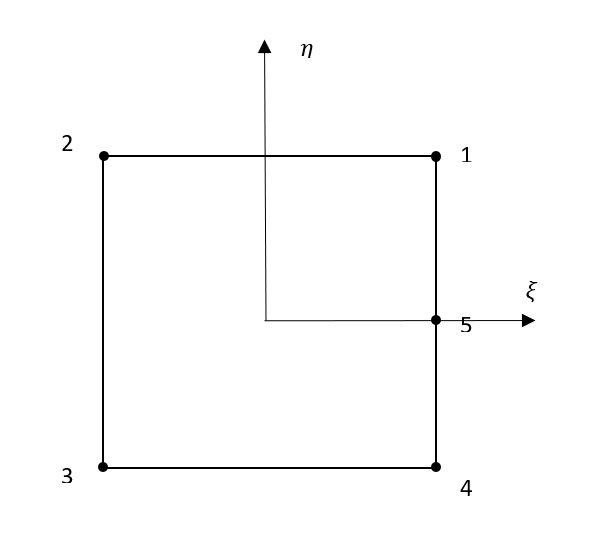
\includegraphics[width=0.6\textwidth,center]{fig/cap6_1_a.PNG}
	\caption{Questão a)} 
	\label{cap6:cap6_1_a}
\end{figure}
\end{itemize}
%
As funções de interpolação serão definidas através das funções bilineares. Considerando a Figura \ref{cap6:quad_bilinear_0}, 
%
\begin{figure}[H]
	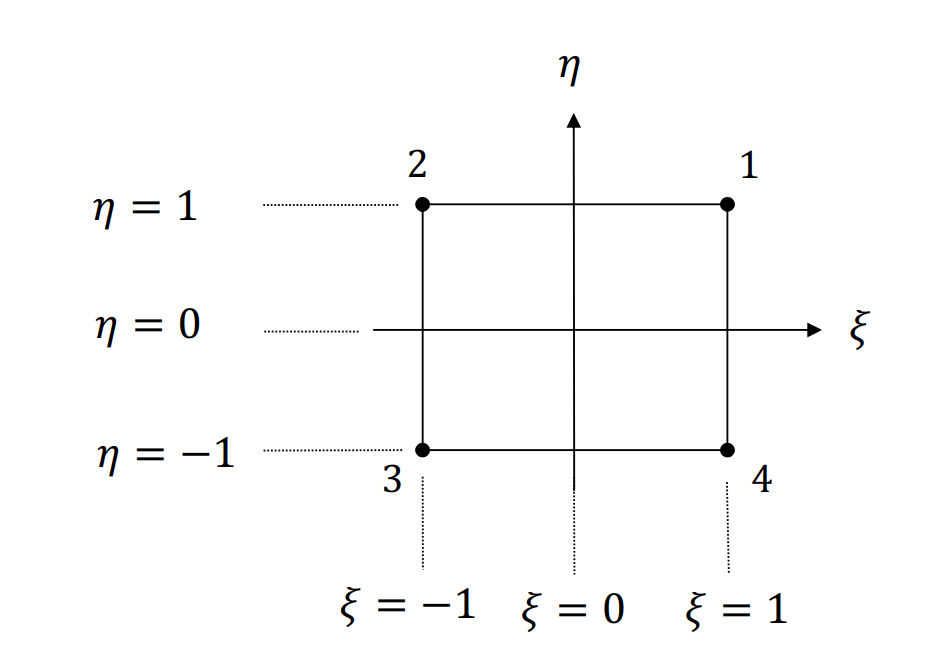
\includegraphics[width=0.6\textwidth,center]{fig/quadrilatero_4_livro.PNG}
	\caption{Parametrização de um elementos quadrilátero bilinear (4 nós)} 
	\label{cap6:quad_bilinear_0}
\end{figure}
%
as funções de interpolações bilineares são,
%
\begin{equation}
	\begin{split}
		&N^b_1(\xi, \eta) = \frac{1}{4}(1 + \xi)(1 + \eta)\\
		&N^b_2(\xi, \eta) = \frac{1}{4}(1 - \xi)(1 + \eta)\\
		&N^b_3(\xi, \eta) = \frac{1}{4}(1 - \xi)(1 - \eta)\\
		&N^b_4(\xi, \eta) = \frac{1}{4}(1 + \xi)(1 - \eta)
	\end{split}
\end{equation}
%
A função de interpolação no ponto 5 é definida como a variação quadrática na direção $\eta$ e linear na direção $\xi$ (Pag. 53). A variação quadrática é obtida pelo polinômio de Lagrange quadrático. Na figura \ref{cap6:Quadratico} temos o elemento que gera a variação quadrática.
%
\begin{figure}[H]
	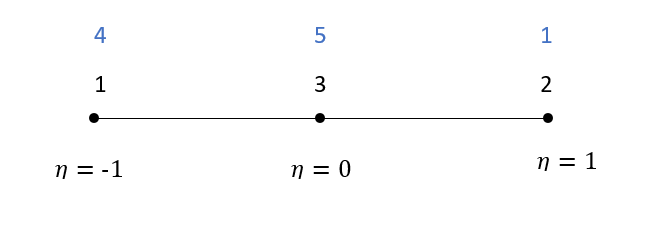
\includegraphics[width=0.6\textwidth,center]{fig/elemento_quad.PNG}
	\caption{Função de interpolação quadrática} 
	\label{cap6:Quadratico}
\end{figure}
%

Na figura \ref{cap6:Quadratico} o ponto 5 equivale ao 3, portanto a variação quadrática é (pag. 49),
%
\begin{equation}
	l^2_3(\eta) = (1-\eta)(1+\eta)
\end{equation}
%
Na variação linear na direção $\xi$ o ponto 5 equivale ao 2 (pag. 49),
%
\begin{equation}
	l^1_2(1+\xi) = \frac{1}{2}(1+\xi)
\end{equation}
%
Assim, o função de interpolação $N_5$ é dada por,
%
\begin{equation}
	N_5(\xi,\eta) = \frac{1}{2}(1+\xi)(1-\eta)(1+\eta)
\end{equation}
%
Usando a lógica das funções de interpolação do elemento de Serendipity (pag. 53). As  funções de interpolação $N_1$ e $N_4$ são as funções de de interpolação bilineares menos ${1/2}$ da função de interpolação no intermediário, no caso o nó 5. Assim temos,
%
\begin{equation}
	\begin{split}
	&N_1(\xi,\eta) = N^b_1(\xi,\eta) - \frac{1}{2}  N_5(\xi,\eta)\\
	&N_4(\xi,\eta) = N^b_4(\xi,\eta) - \frac{1}{2}  N_5(\xi,\eta)
	\end{split}
\end{equation}
%	
As aresta do nós 2 e 3 não possuem nós intermediários, portanto as função são as função bilineares. 

\color{blue}
\textbf{Resposta:}
\begin{equation}
	\begin{split}
		&N_1(\xi,\eta) = N^b_1(\xi,\eta) - \frac{1}{2}  N_5(\xi,\eta)\\
		&N_2(\xi,\eta) = N^b_2(\xi,\eta)\\
		&N_3(\xi,\eta) = N^b_3(\xi,\eta)\\
		&N_4(\xi,\eta) = N^b_4(\xi,\eta) - \frac{1}{2}  N_5(\xi,\eta)\\
		&N_5(\xi,\eta) = \frac{1}{2}(1+\xi)(1-\eta)(1+\eta)\\
	\end{split}
\end{equation}
\color{black}

\subsubsection{Calcular o operador Jacobiano dos seguintes elementos}

O Jacobiano 2D é definido por:
%
\begin{equation}
	J(\xi, \eta) = 
	\begin{bmatrix}
		\mdp{x}{\xi} & \mdp{y}{\xi}\\
		\mdp{x}{\eta} & \mdp{y}{\eta}\\
	\end{bmatrix}
\end{equation}
%
Todos os elementos são quadriláteros de 4 nós, assim a interpolação geométrica é dada por
%
\begin{equation}
	\begin{split}
		&x(\xi, \eta) = x_1 N_1(\xi, \eta) + x_2 N_2(\xi, \eta) + x_3 N_3(\xi, \eta) + x_4 N_4(\xi, \eta)\\
		&y(\xi, \eta) = y_1 N_1(\xi, \eta) + y_2 N_2(\xi, \eta) + y_3 N_3(\xi, \eta) + y_4 N_4(\xi, \eta)
	\end{split}
\end{equation}
%
Considerando a Figura \ref{cap6:quad_bilinear}, 
%
\begin{figure}[H]
	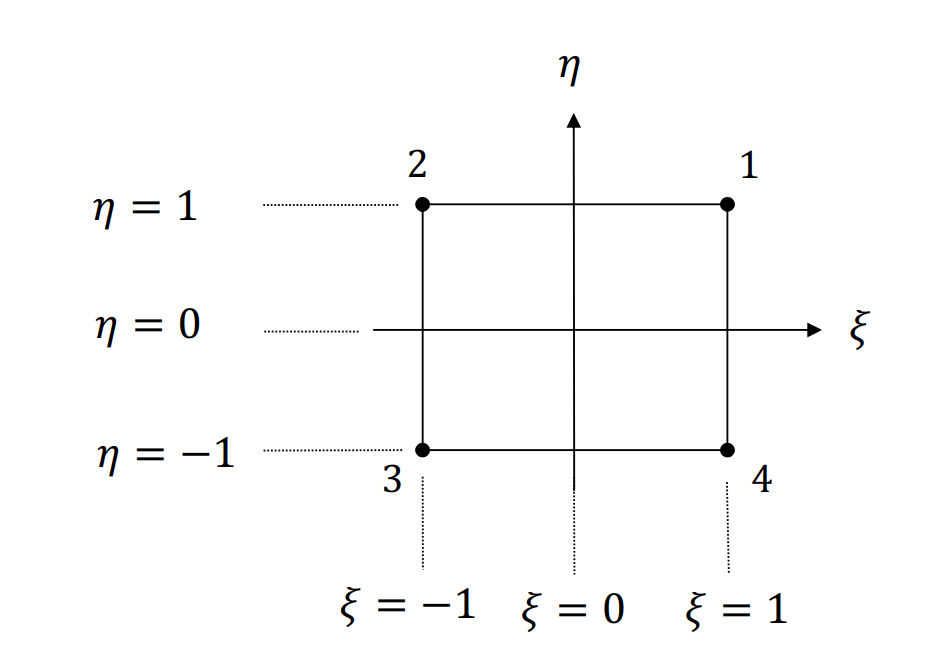
\includegraphics[width=0.6\textwidth,center]{fig/quadrilatero_4_livro.PNG}
	\caption{Parametrização de um elementos quadrilátero bilinear (4 nós)} 
	\label{cap6:quad_bilinear}
\end{figure}
%
as funções de interpolações bilineares são,
%
\begin{equation}
	\begin{split}
		&N_1(\xi, \eta) = \frac{1}{4}(1 + \xi)(1 + \eta)\\
		&N_2(\xi, \eta) = \frac{1}{4}(1 - \xi)(1 + \eta)\\
		&N_3(\xi, \eta) = \frac{1}{4}(1 - \xi)(1 - \eta)\\
		&N_4(\xi, \eta) = \frac{1}{4}(1 + \xi)(1 - \eta)
	\end{split}
\end{equation}
%
A as derivadas em relação a $\xi$ são,
\begin{equation}
	\begin{split}
		&\mdp{N_1}{\xi} = \frac{1}{4}(1 + \eta)\\
		&\mdp{N_2}{\xi} =-\frac{1}{4}(1 + \eta)\\
		&\mdp{N_3}{\xi} =-\frac{1}{4}(1 - \eta)\\
		&\mdp{N_4}{\xi} = \frac{1}{4}(1 - \eta)\\
	\end{split}
\end{equation}
%
e as derivadas em relação a $\eta$ são,
\begin{equation}
	\begin{split}
		&\mdp{N_1}{\eta} = \frac{1}{4}(1 + \xi)\\
		&\mdp{N_2}{\eta} = \frac{1}{4}(1 - \xi)\\
		&\mdp{N_3}{\eta} =-\frac{1}{4}(1 - \xi)\\
		&\mdp{N_4}{\eta} =-\frac{1}{4}(1 + \xi)\\
	\end{split}
\end{equation}
%
A deriva de $x$ em relação a  $\xi$ são,
%
\begin{equation}
	\begin{split}
&	\mdp{x}{\xi} = x_1 \mdp{N_1}{\xi} + x_2 \mdp{N_2}{\xi} + x_3 \mdp{N_3}{\xi} + x_4 \mdp{N_4}{\xi}\\
&   \mdp{x}{\xi} = \frac{x_1}{4} (1 + \eta) - \frac{x_2}{4} (1 + \eta) - \frac{x_1}{4} (1 - \eta) + \frac{x_4}{4} (1 - \eta)\\
&   \mdp{x}{\xi} = \frac{1}{4}\left[ (x_1 - x_2)(1 + \eta) + (x_4 - x_3)(1 - \eta) \right]
	\end{split}
\end{equation}
%
A deriva de $y$ em relação a  $\xi$ são,
%
\begin{equation}
	\begin{split}
		&	\mdp{y}{\xi} = y_1 \mdp{N_1}{\xi} + y_2 \mdp{N_2}{\xi} + y_3 \mdp{N_3}{\xi} + y_4 \mdp{N_4}{\xi}\\
		&   \mdp{y}{\xi} = \frac{1}{4}\left[ (y_1 - y_2)(1 + \eta) + (y_4 - y_3)(1 - \eta) \right]
	\end{split}
\end{equation}
%
A deriva de $x$ em relação a  $\eta$ são,
%
\begin{equation}
	\begin{split}
		&	\mdp{x}{\eta} = x_1 \mdp{N_1}{\eta} + x_2 \mdp{N_2}{\eta} + x_3 \mdp{N_3}{\eta} + x_4 \mdp{N_4}{\eta}\\
		&   \mdp{x}{\eta} = \frac{1}{4}\left[ (x_1 - x_4)(1 + \xi) + (x_2 - x_3)(1 - \xi) \right]
	\end{split}
\end{equation}
%
A deriva de $y$ em relação a  $\eta$ são,
%
\begin{equation}
	\begin{split}
		&	\mdp{y}{\eta} = y_1 \mdp{N_1}{\eta} + y_2 \mdp{N_2}{\eta} + y_3 \mdp{N_3}{\eta} + y_4 \mdp{N_4}{\eta}\\
		&   \mdp{y}{\eta} = \frac{1}{4}\left[ (y_1 - y_4)(1 + \xi) + (y_2 - y_3)(1 - \xi) \right]
	\end{split}
\end{equation}
%
Assim o operador jacobiano fica definido como,
%
\begin{equation}
	\begin{split}
&	\mdp{x}{\xi } = \frac{1}{4}\left[ (x_1 - x_2)(1 + \eta) + (x_4 - x_3)(1 - \eta) \right]\\
&   \mdp{y}{\xi } = \frac{1}{4}\left[ (y_1 - y_2)(1 + \eta) + (y_4 - y_3)(1 - \eta) \right]\\
&   \mdp{x}{\eta} = \frac{1}{4}\left[ (x_1 - x_4)(1 + \xi ) + (x_2 - x_3)(1 - \xi ) \right]\\
&   \mdp{y}{\eta} = \frac{1}{4}\left[ (y_1 - y_4)(1 + \xi ) + (y_2 - y_3)(1 - \xi ) \right]
	\end{split}
\end{equation}
%
Resolvendo agora as questões:
%
\begin{itemize}
	\item a)
	Considerando o ponto $P_3$ como referencia, temos as seguintes coordenadas para os pontos,
	%
	\begin{equation}
		\begin{split}
			&	P_1 = (x_3 + 6, y_3 + 4)\\
			&	P_2 = (x_3    , y_3 + 4)\\
			&	P_3 = (x_3    , y_3    )\\
			&	P_4 = (x_3 + 6, y_3    )\\
		\end{split}
	\end{equation}
	%
	Nos temos agora que para os $xs$,
	\begin{equation}
		\begin{split}
			&	(x_1 - x_2) = x_3 + 6 - x_3 = 6 \\
			&	(x_4 - x_3) = x_3 + 6 - x_3 = 6\\
			&	(x_1 - x_4) = x_3 + 6 - (x_3 + 6) = 0\\\
			&	(x_2 - x_3) = x_3 - x_3 = 0\\
		\end{split}
	\end{equation}
	%
	e para os $ys$,
	\begin{equation}
	\begin{split}
		&	(y_1 - y_2) = y_3 + 4 - (y_3 + 4) = 0 \\
		&	(y_4 - y_3) = y_3 - y_3 = 0\\
		&	(y_1 - y_4) = y_3 + 4 - y_3 = 4\\\
		&	(y_2 - y_3) = y_3 + 4 - y_3 = 4\\
	\end{split}
	\end{equation}
	%
	\begin{equation}
		\begin{split}
			&	\mdp{x}{\xi } = \frac{1}{4}\left[ 6(1 + \eta) + 6(1 - \eta) \right] = 3\\
			&   \mdp{y}{\xi } = \frac{1}{4}\left[ 0(1 + \eta) + 0(1 - \eta) \right] = 0\\
			&   \mdp{x}{\eta} = \frac{1}{4}\left[ 0(1 + \xi ) + 0(1 - \xi ) \right] = 0\\
			&   \mdp{y}{\eta} = \frac{1}{4}\left[ 4(1 + \xi ) + 4(1 - \xi ) \right] = 2
		\end{split}
	\end{equation}
	%
	Portando o operador Jacobiano é dado por,

	\color{blue}
	\textbf{Resposta:}
	\begin{equation}
	J(\xi, \eta) = 
	\begin{bmatrix}
		3 & 0\\
		0 & 2\\
	\end{bmatrix}
	\end{equation}	
	\color{black}
	% 
	Pode-se checar o resultado através do calculo da área do elemento,
	\begin{equation}
		\begin{split}
		& A = b * h = \int_A dA = \int_{-1}^1 \int_{-1}^1 det J d\xi d\eta\\
		& 4 * 6 = \int_{-1}^1 \int_{-1}^1 \left(3 * 2\right)  d\xi d\eta\\
		& 4 * 6 = 6 * 2 * 2 \\
		& 24 = 24		
		\end{split}
	\end{equation}
	%	
\end{itemize}

\subsubsection{Calcular as forças nodais equivalentes para os elementos de elasticidades plana abaixo, considerando uma distribuição uniforme de forças de volume na direção y}

A integral de forças de volume é(pag. 22),
%
\begin{equation}
\mathbf{f}_i = \int_{\Omega} \mathbf{N}_i \mathbf{b} d\Omega
\end{equation}
%
em notação matricial temos,
%
\begin{equation}
	\begin{bmatrix}
	f^x_i\\
	f^y_i\\
	\end{bmatrix}
	=
	\int_{\Omega}
	\begin{bmatrix}
	N_i&0\\
	0&N_i\\
	\end{bmatrix}
	\begin{bmatrix}
	b_x\\
	b_y\\
	\end{bmatrix}
	d\Omega
	=
	\int_{\Omega}
	\begin{bmatrix}
		N_i b_x\\
		N_i b_y\\
	\end{bmatrix}
	d\Omega
	=
	\begin{bmatrix}
	\int_{\Omega} N_i b_x d\Omega\\
	\int_{\Omega} N_i b_y d\Omega\\
	\end{bmatrix}
\end{equation}
%
Como $b_x$ é igual 0, temos,
%
\begin{equation}
	\begin{bmatrix}
		f^x_i\\
		f^y_i\\
	\end{bmatrix}
	=
	\begin{bmatrix}
		0\\
		\int_{\Omega} N_i b_y d\Omega\\
	\end{bmatrix}
\end{equation}
%
É necessário calcular a integral em relação a $N_i$, lembrando que a integral é em relação ao sistema de coordenadas x-y,
%
\begin{equation}
\int_{\Omega} N_i(x,y) d\Omega
\end{equation}
%
A integral usando as coordenadas locais no elemento triangular é,
%
\begin{equation}
	\int_{\Omega} N_i(x,y) d\Omega = \int_{0}^{1} \int_{0}^{1-\xi_1}  N_i(\xi_1,\xi_2) det J d \xi_1 d \xi_2 
\end{equation}
%
Considerando uma interpolação linear para geometria o determinante do jacobiano é constante e igual a duas vezes a área do triangulo, portando,
%
\begin{equation}
	\int_{\Omega} N_i(x,y) d\Omega = 2 A \int_{0}^{1} \int_{0}^{1-\xi_1}  N_i(\xi_1,\xi_2) d \xi_1 d \xi_2 = 2 A f_i
\end{equation}
%
Para resolver o problema precisamos apenas calcular essas integrais.

\begin{itemize}
	\item a)
	Para o triangulo linear temos as seguintes funções de interpolação
	%
	\begin{equation}
		\begin{split}
		&N_1 = \xi_1\\ 
		&N_2 = \xi_2\\ 
		&N_3 = 1 - \xi_1 - \xi_2\\ 
		\end{split}
	\end{equation}
	%	
	A integrais ficam
	%
	\begin{equation}
		\begin{split}
			&f_1 = \int_{0}^{1} \int_{0}^{1-\xi_1}  N_1 d \xi_1 d \xi_2 = \int_{0}^{1} \int_{0}^{1-\xi_1}  \xi_1 d \xi_1 d \xi_2 = \frac{1}{6}\\ 
			&f_2 = \int_{0}^{1} \int_{0}^{1-\xi_1}  N_2 d \xi_1 d \xi_2 = \int_{0}^{1} \int_{0}^{1-\xi_1}  \xi_2 d \xi_1 d \xi_2 = \frac{1}{6}\\ 
			&f_3 = \int_{0}^{1} \int_{0}^{1-\xi_1}  N_3 d \xi_1 d \xi_2 = \int_{0}^{1} \int_{0}^{1-\xi_1}  1 - \xi_1 - \xi_2 d \xi_1 d \xi_2 = \frac{1}{6} 
		\end{split}
	\end{equation}
	%
	Portanto
	\begin{equation}
		\begin{split}
			&f_1^y = (b_y) (2 A) \left(\frac{1}{6}\right) = \frac{b_y A}{3}\\ 
			&f_2^y = (b_y) (2 A) \left(\frac{1}{6}\right) = \frac{b_y A}{3}\\ 
			&f_3^y = (b_y) (2 A) \left(\frac{1}{6}\right) = \frac{b_y A}{3} 
		\end{split}
	\end{equation}
	% 
	Assim os vetores de força equivalentes é dados por,

	\color{blue}
	\textbf{Resposta:}
	\begin{equation}
		\mathbf{f}_1 = \mathbf{f}_2 = \mathbf{f}_3
		=
		\frac{b_y A}{3}
		\begin{bmatrix}
			0\\
			1
		\end{bmatrix}
	\end{equation}
	\color{black}
	%
	
	\item b)
	Para o triangulo quadrático temos as seguintes funções de interpolação
	%
	\begin{equation}
		\begin{split}
			&N_1 = \xi_1(2\xi_1 - 1)\\ 
			&N_2 = \xi_2(2\xi_2 - 1)\\ 
			&N_3 = \xi_3(2\xi_3 - 1)\\ 
			&N_4 = 4 \xi_1 \xi_2\\ 
			&N_5 = 4 \xi_2 \xi_3\\ 
			&N_6 = 4 \xi_3 \xi_1 
		\end{split}
	\end{equation}
	%	
	A integrais ficam
	%
	\begin{equation}
		\begin{split}
			&f_1 = \int_{0}^{1} \int_{0}^{1-\xi_1}  N_1 d \xi_1 d \xi_2 = 0\\ 
			&f_2 = \int_{0}^{1} \int_{0}^{1-\xi_1}  N_2 d \xi_1 d \xi_2 = 0\\ 
			&f_3 = \int_{0}^{1} \int_{0}^{1-\xi_1}  N_3 d \xi_1 d \xi_2 = 0\\ 
			&f_4 = \int_{0}^{1} \int_{0}^{1-\xi_1}  N_1 d \xi_1 d \xi_2 = \frac{1}{6}\\ 
			&f_5 = \int_{0}^{1} \int_{0}^{1-\xi_1}  N_2 d \xi_1 d \xi_2 = \frac{1}{6}\\ 
			&f_6 = \int_{0}^{1} \int_{0}^{1-\xi_1}  N_3 d \xi_1 d \xi_2 = \frac{1}{6} 
		\end{split}
	\end{equation}
	%	
	Portanto
	\begin{equation}
	\begin{split}
		&f_1^y = 0\\ 
		&f_2^y = 0\\ 
		&f_3^y = 0\\
		&f_4^y = \frac{b_y A}{3}\\ 
		&f_5^y = \frac{b_y A}{3}\\ 
		&f_6^y = \frac{b_y A}{3}  
	\end{split}
	\end{equation}
	% 
	Assim os vetores de força equivalentes é dados por,

	\color{blue}
	\textbf{Resposta:}
	\begin{equation}
	\begin{split}
		&\mathbf{f}_1 = \mathbf{f}_2 = \mathbf{f}_3 =
		\begin{bmatrix}
			0\\
			0
		\end{bmatrix}\\
		&\mathbf{f}_4 = \mathbf{f}_5 = \mathbf{f}_6  
		=
		\frac{b_y A}{3}
		\begin{bmatrix}
			0\\
			1
		\end{bmatrix}
		\end{split}
	\end{equation}
	\color{black}
%
%
\end{itemize}

\subsubsection{Calcular as forças nodais equivalentes para os elementos quadriláteros quadrático de elasticidade plana}

A integral de forças de volume é(pag. 22),
%
\begin{equation}
	\mathbf{f}_i = \int_{\Gamma} \mathbf{N}_i \mathbf{\bar t} d\Gamma
\end{equation}
%
em notação matricial temos,
%
\begin{equation}
	\begin{bmatrix}
		f^x_i\\
		f^y_i\\
	\end{bmatrix}
	=
	\int_{\Gamma}
	\begin{bmatrix}
		N_i&0\\
		0&N_i\\
	\end{bmatrix}
	\begin{bmatrix}
		q_x\\
		q_y\\
	\end{bmatrix}
	d\Gamma
	=
	\int_{\Gamma}
	\begin{bmatrix}
		N_i t_x\\
		N_i t_y\\
	\end{bmatrix}
	d\Gamma
	=
	\begin{bmatrix}
		\int_{\Gamma} N_i t_x d\Gamma\\
		\int_{\Gamma} N_i t_y d\Gamma
	\end{bmatrix}
\end{equation}
%
Como a força são uniformes nos bordos,
%
\begin{equation}
	\begin{bmatrix}
		f^x_i\\
		f^y_i\\
	\end{bmatrix}
	=
	\begin{bmatrix}
		t_x \int_{\Gamma} N_i d\Gamma\\
		t_y \int_{\Gamma} N_i d\Gamma
	\end{bmatrix}
\end{equation}
%
Portanto temos,
%
\begin{equation}
\begin{split}
&f^x_2 = t_x \int_{\Gamma} N_2 d\Gamma \quad f^y_2 = 0\\
&f^x_6 = t_x \int_{\Gamma} N_6 d\Gamma \quad f^y_6 = 0\\
&f^x_3 = t_x \int_{\Gamma} N_3 d\Gamma \quad f^y_3 =  t_y \int_{\Gamma} N_3 d\Gamma\\
&f^x_7 = 0 \quad f^y_7 =  t_y \int_{\Gamma} N_7 d\Gamma\\
&f^x_4 = 0 \quad f^y_4 = t_y \int_{\Gamma} N_4 d\Gamma
\end{split}
\end{equation}
%
Como a integral é apenas nos bordos, na aresta 2-3 temos, as seguintes funções de interpolações 
%
\begin{equation}
	\begin{split}
		&N_2 = \frac{1}{2} \eta (1 + \eta) \\ 
		&N_6 = \eta (1 - \eta) (1 + \eta) \\ 
		&N_3 = -\frac{1}{2} \eta (1 - \eta)  
	\end{split}
\end{equation}
%
As integrais são,
\begin{equation}
	\begin{split}
		&\int_{\Gamma} N_2 d\Gamma = \int_{-1}^{1} N_2 det J d\eta = \frac{L}{2} \int_{-1}^{1} N_2 d\eta =  \frac{L}{6}\\
		&\int_{\Gamma} N_6 d\Gamma = \int_{-1}^{1} N_6 det J d\eta = \frac{L}{2} \int_{-1}^{1} N_6 d\eta =  \frac{2 L}{3}\\
		&\int_{\Gamma} N_3 d\Gamma = \int_{-1}^{1} N_3 det J d\eta = \frac{L}{2} \int_{-1}^{1} N_3 d\eta =  \frac{L}{6}
	\end{split}
\end{equation}
Como a integral é apenas nos bordos, na aresta 3-4 temos, as seguintes funções de interpolações 
%
\begin{equation}
	\begin{split}
		&N_3 = -\frac{1}{2} \xi (1 - \xi) \\ 
		&N_7 = \xi (1 - \xi) (1 + \xi) \\ 
		&N_4 = \frac{1}{2} \xi (1 + \xi)  
	\end{split}
\end{equation}
%
As integrais são,
\begin{equation}
	\begin{split}
		&\int_{\Gamma} N_3 d\Gamma = \int_{-1}^{1} N_3 det J d\eta = \frac{L}{2} \int_{-1}^{1} N_3 d\eta =  \frac{L}{6}\\
		&\int_{\Gamma} N_7 d\Gamma = \int_{-1}^{1} N_7 det J d\eta = \frac{L}{2} \int_{-1}^{1} N_7 d\eta =  \frac{2 L}{3}\\
		&\int_{\Gamma} N_4 d\Gamma = \int_{-1}^{1} N_4 det J d\eta = \frac{L}{2} \int_{-1}^{1} N_4 d\eta =  \frac{L}{6}
	\end{split}
\end{equation}
%
Portanto temos,
%
\begin{equation}
	\begin{split}
		&f^x_2 = \frac{t_x L}{6} \quad f^y_2 = 0\\
		&f^x_6 = \frac{2 t_x L}{3} \quad f^y_6 = 0\\
		&f^x_3 = \frac{t_x L}{6} \quad f^y_3 = \frac{t_y L}{6}\\
		&f^x_7 = 0 \quad f^y_7 = \frac{2 t_y L}{3}\\
		&f^x_4 = 0 \quad f^y_4 = \frac{t_y L}{6}
	\end{split}
\end{equation}
%
\color{blue}
\textbf{Resposta:}
\begin{equation}
	\begin{split}
		&\mathbf{f}_2 =
		\begin{bmatrix}
			\frac{t_x L}{6}\\
			0
		\end{bmatrix}\\
		&\mathbf{f}_3 =
		\begin{bmatrix}
		\frac{t_x L}{6}\\
		\frac{t_y L}{6}
		\end{bmatrix}\\
		&\mathbf{f}_4 =
		\begin{bmatrix}
		0\\
		\frac{t_y L}{6}
		\end{bmatrix}\\
		&\mathbf{f}_6 =
		\begin{bmatrix}
		\frac{2 t_x L}{3}\\
		0
		\end{bmatrix}\\
		&\mathbf{f}_7 =
		\begin{bmatrix}
		0\\
		\frac{2 t_y L}{3}
		\end{bmatrix}
	\end{split}
\end{equation}
\color{black}



\section{Operadores Diferencias}
%
\subsection{Gradiente}
%
O operado diferencial gradiente é definido por,
%
\begin{equation}
	grad() = \bar \nabla() = \frac{\partial()}{\partial x} \pmb{\hat i} + \frac{\partial()}{\partial y} \pmb{\hat j} + \frac{\partial()}{\partial z} \pmb{\hat z} = \left[\frac{\partial()}{\partial x}\; \frac{\partial()}{\partial y}\; \frac{\partial()}{\partial z}  \right]
\end{equation}
%
O gradiente de um escalar é um vetor, por exemplo, o gradiente de $u$ é um vetor dados por,
%
\begin{equation}
	\bar \nabla(u) = \frac{\partial u}{\partial x} \pmb{\hat i} + \frac{\partial u}{\partial y} \pmb{\hat j} + \frac{\partial u }{\partial z} \pmb{\hat z}
\end{equation}
%
Uma aplicação prática do gradiente é fluxo de calor que é dado pelo gradiente da Temperatura:
%
\begin{equation}
	\bar q = - k \bar \nabla(T) = - k \left(\frac{\partial T}{\partial x} \pmb{\hat i} + \frac{\partial T}{\partial y} \pmb{\hat j} + \frac{\partial T}{\partial T} \pmb{\hat z}\right)
\end{equation}
%
Outra forma de escrever o gradiente é usando notação indicial
%
\begin{equation}
	\bar \nabla(u) = \frac{\partial u}{\partial x_1} \pmb{\hat i_1} + \frac{\partial u}{\partial x_2} \pmb{\hat i_2} + \frac{\partial u}{\partial x_3} \pmb{\hat i_3} = \sum_{j = 1}^3 \frac{\partial u}{\partial x_j} \pmb{\hat i_j} =  \frac{\partial u}{\partial x_j} \pmb{\hat i_j} = u_{,j} \pmb{\hat i_j}
\end{equation}
%
\subsection{Divergente}
%
O operado diferencial divergente é definido por,
%
\begin{equation}
	div() = \bar \nabla \bullet () = \frac{\partial()}{\partial x} + \frac{\partial()}{\partial y} + \frac{\partial()}{\partial z} 
\end{equation}
%
Por exemplo, considere o vetor velocidade $\pmb{\bar v}$ dado por,
%
\begin{equation}
	\pmb{\bar v} =	u \pmb{\hat i} + v \pmb{\hat j} + w \pmb{\hat z}
\end{equation}
%
O divergente é dado,
%
\begin{equation}
	\bar \nabla \bullet \pmb{\bar v} = \frac{\partial u}{\partial x} + \frac{\partial v}{\partial y} + \frac{\partial w}{\partial z} 
\end{equation}
%
Em notação indicial a velocidade fica,
%
\begin{equation}
	\pmb{\bar v} =	u_1 \pmb{\hat i_1} + u_2 \pmb{\hat i_2} + u_3 \pmb{\hat i_3}
\end{equation}
%
E o divergente
%
\begin{equation}
	\bar \nabla \bullet \pmb{\bar v} = \frac{\partial u_1}{\partial x_1} + \frac{\partial u_2}{\partial x_2} + \frac{\partial u_3}{\partial x_3} = \frac{\partial u_j}{\partial x_j} = u_{j,j}
\end{equation}
%
\subsection{Operado laplaciano}
%
O operado laplaciano é o divergente do gradiente,
\begin{equation}
	div(grad()) = \bar \nabla \bullet \bar \nabla() = \frac{\partial^2()}{\partial x^2} + \frac{\partial^2()}{\partial y^2} + \frac{\partial^2()}{\partial z^2} = \nabla^2 ()
\end{equation}





\section{Teorema do divergente}

A teorema do divergente é dado por:
%
\begin{equation}
	\int_{\Omega} \nabla \bullet \pmb{\bar F} d \Omega = \int_{\Gamma} \pmb{\bar F} \bullet \pmb{\bar n} d \Gamma
\end{equation} 
%
O vetor $\pmb{\bar F}$ e  $\pmb{\bar n}$ podem ser escritos como,
%
\begin{equation}
	\begin{split}
	&\pmb{\bar F} = \left(F_x, F_y, F_z\right)\\
	&\pmb{\bar n} = \left(n_x, n_y, n_z\right)
	\end{split}
\end{equation} 
%
Assim da para escrever o teorema do divergente como,
%
\begin{equation}
\int_{\Omega} \left(\mdp{F_x}{x} + \mdp{F_y}{y} + \mdp{F_z}{z}\right) d \Omega = \int_{\Gamma} \left(F_x n_x + F_y n_y + F_z n_z\right) d \Gamma
\end{equation}
%
Pode-se provar ainda que,
%
\begin{equation}
	\begin{split}
		&\int_{\Omega} \mdp{F_x}{x} d \Omega = \int_{\Gamma} F_x n_x d \Gamma\\
		&\int_{\Omega} \mdp{F_y}{y} d \Omega = \int_{\Gamma} F_y n_y d \Gamma\\
		&\int_{\Omega} \mdp{F_z}{z} d \Omega = \int_{\Gamma} F_z n_z d \Gamma
	\end{split}
\end{equation} 
%
Considerando que $F_x = \mdp{\phi}{x} w$, $F_y = \mdp{\phi}{y} w$ e $F_z = \mdp{\phi}{z} w$ nos temos,
%
\begin{equation}
	\begin{split}
		&\int_{\Omega} \mdp{}{x}\left(\mdp{\phi}{x} w\right) d \Omega = \int_{\Gamma} \mdp{\phi}{x} w \, n_x d \Gamma\\
		&\int_{\Omega} \mdp{}{y}\left(\mdp{\phi}{y} w\right) d \Omega = \int_{\Gamma} \mdp{\phi}{y} w \,n_y d \Gamma\\
		&\int_{\Omega} \mdp{}{z}\left(\mdp{\phi}{z} w\right) d \Omega = \int_{\Gamma} \mdp{\phi}{z} w \,n_z d \Gamma
	\end{split}
\end{equation} 
%
\section{Equação de transferência de calor }
%
A equação de calor é dada por,
%
\begin{equation}
	\frac{\partial( \rho c_p T )}{\partial t} = \bar \nabla \bullet ( k \bar \nabla T ) + Q(x, y, z, t)
\end{equation}
%
onde $\rho$ é massa especifica, $c_p$ é o calor especifico, $k$ é coeficiente de condutividade térmica e $Q(x, y, z, t)$ é um termo fonte de geração de calor.  
%
Considerando o regime permanente temos,
%
\begin{equation}
	\bar \nabla \bullet ( k \bar \nabla T ) + Q(x, y, z) = 0
\end{equation}
%
Agora considerando que o $k$ é constante,
%
\begin{equation}
	\begin{split}
		k\left(\bar \nabla \bullet \bar \nabla T\right) + Q(x, y, z) = 0\\	 
		k \nabla^2 T + Q(x, y, z) = 0
	\end{split}
\end{equation}
%
Dividindo $k$
%
\begin{equation}
	\begin{split}
		\nabla^2 T = -Q(x, y, z)/ k = 0\\	 
		\nabla^2 T = Q^*(x, y, z)
	\end{split}
\end{equation}
%
A equação abaixo é conhecida com Equação de Poisson
%
\begin{equation}
	\nabla^2 T = \frac{\partial^2 T}{\partial x^2} + \frac{\partial^2 T}{\partial y^2} + \frac{\partial^2 T}{\partial z^2} = Q^*(x, y, z)	
\end{equation}
%
A equação de Laplace é a equação de Poisson com termo fonte nulo,
%
\begin{equation}
	\nabla^2 T = \frac{\partial^2 T}{\partial x^2} + \frac{\partial^2 T}{\partial y^2} + \frac{\partial^2 T}{\partial z^2} = 0
\end{equation}
%
Para um problema 1D a equações de Poisson fica,
%
\begin{equation}
	\frac{\partial^2 T}{\partial x^2} = \frac{d^2 T}{d x^2} = Q^*(x)	
\end{equation}
%
%
\section{Equação de transporte de calor }
%
A equação de transporte de calor é dada por,
%
\begin{equation}
	\frac{\partial( \rho c_p T )}{\partial t} + \bar \nabla \bullet (\rho c_p \pmb{\bar v} T ) = \bar \nabla \bullet ( k \bar \nabla T ) + Q(x, y, z, t)
\end{equation}
\section{Exercícios extras}

\subsection{Q3 - prova - 2010}

A matriz $\mathbf{B}$ é dada por,

\begin{equation}
	\mathbf{B} =
	\begin{bmatrix}
	\mathbf{B}_1&  \mathbf{B}_2& \mathbf{B}_3
	\end{bmatrix}
\end{equation} 

onde as matrizes $\mathbf{B}_1$, $\mathbf{B}_2$ e $\mathbf{B}_3$ são dadas por,
%
\begin{equation}
	\mathbf{B_1} = \pounds \mathbf{N}_1 = 
	\begin{bmatrix}
		\mdp{N_1}{x}& 0\\
    	           0& \mdp{N_1}{y}\\
		\mdp{N_1}{y}& \mdp{N_1}{x}
	\end{bmatrix}
\end{equation}
%
\begin{equation}
	\mathbf{B_2} = \pounds \mathbf{N}_2 = 
	\begin{bmatrix}
		\mdp{N_2}{x}& 0\\
		0& \mdp{N_2}{y}\\
		\mdp{N_2}{y}& \mdp{N_2}{x}
	\end{bmatrix}
\end{equation}
%
\begin{equation}
	\mathbf{B_3} = \pounds \mathbf{N}_3 = 
	\begin{bmatrix}
		\mdp{N_3}{x}& 0\\
		0& \mdp{N_3}{y}\\
		\mdp{N_3}{y}& \mdp{N_3}{x}
	\end{bmatrix}
\end{equation}
%
Agora temos que calcular as derivadas das funções de interpolação. A relação entre as derivas em relação a $x$ e $y$ com as coordenadas locais $\xi_1$ e $\xi_2$ é dada pela inversa da matriz Jacobiana.
%
\begin{equation}
	\begin{bmatrix}
		\mdp{}{x}\\
		\mdp{}{y}
	\end{bmatrix} = J^{-1} 
	\begin{bmatrix}
	\mdp{}{\xi_1}\\
	\mdp{}{\xi_2}	
	\end{bmatrix}
	\label{provas:derivada_jacobiano}
\end{equation}
%
Para calcular a matriz inversa precisamos calcular A matriz Jacobina, para um de um triangulo linear temos,
%
\begin{equation}
J =	\begin{bmatrix}
		\mdp{x}{\xi_1}&\mdp{y}{\xi_1}\\
		\mdp{x}{\xi_2}&\mdp{y}{\xi_2}
	\end{bmatrix} =
    \begin{bmatrix}
  		x_1 - x_3&y_1 - y_3\\
	  	x_2 - x_3&y_2 - y_3
    \end{bmatrix} 
\end{equation}
%
Considerando a figura temos,
\begin{equation}
\begin{split}
x_1 = 1\\
y_1 = 0\\
x_2 = 0\\
y_2 = 1\\
x_3 = 0\\
y_3 = 0
\end{split}
\end{equation} 
% 
Portanto a matriz Jacobiana é dada por,
%
\begin{equation}
	J =	\begin{bmatrix}
		1&0\\
		0&1
		\end{bmatrix}
\end{equation}
%
A matriz inversa de uma matriz identidade é a própria matriz, ou seja,
%
\begin{equation}
	J^{-1} = J =	\begin{bmatrix}
		1&0\\
		0&1
	\end{bmatrix}
\end{equation}
%
Considerando agora a eq. (\ref{provas:derivada_jacobiano}) temos a relação entre as derivas da função $N_1$,
%
\begin{equation}
	\begin{bmatrix}
	\mdp{N_1}{x}\\
	\mdp{N_1}{y}
	\end{bmatrix}
     = 
	\begin{bmatrix}
	1&0\\
	0&1
	\end{bmatrix}          
	\begin{bmatrix}
	\mdp{N_1}{\xi_1}\\
	\mdp{N_1}{\xi_2}
	\end{bmatrix} 
\end{equation}
%
Sendo assim temos,
%
\begin{equation}
	\begin{split}
		\mdp{N_1}{x} = \mdp{N_1}{\xi_1}\\
		\mdp{N_1}{y} = \mdp{N_1}{\xi_2}
	\end{split}
\end{equation}
%
O mesmo raciocínio pode ser aplicado as funções $N_2$ e $N_3$, o que leva à,
%
\begin{equation}
	\begin{split}
		\mdp{N_2}{x} = \mdp{N_2}{\xi_1}\\
		\mdp{N_2}{y} = \mdp{N_2}{\xi_2}\\
		\mdp{N_3}{x} = \mdp{N_3}{\xi_1}\\
		\mdp{N_3}{y} = \mdp{N_3}{\xi_2}
	\end{split}
\end{equation}
%
Para o triangulo linear temos as seguintes funções de interpolação
%
\begin{equation}
	\begin{split}
		&N_1 = \xi_1\\ 
		&N_2 = \xi_2\\ 
		&N_3 = 1 - \xi_1 - \xi_2\\ 
	\end{split}
\end{equation}
%
Assim as derivas são,
%
\begin{equation}
	\begin{split}
		\mdp{N_1}{x} = 1\\
		\mdp{N_1}{y} = 0\\
		\mdp{N_2}{x} = 0\\
		\mdp{N_2}{y} = 1\\
		\mdp{N_3}{x} = -1\\
		\mdp{N_3}{y} = -1
	\end{split}
\end{equation}
%
A matriz $\mathbf{B}_1$, $\mathbf{B}_2$ e $\mathbf{B}_3$ ficam definidas como,
%
\begin{equation}
	\mathbf{B_1} = \pounds \mathbf{N}_1 = 
	\begin{bmatrix}
		1& 0\\
		0& 0\\
		0& 1
	\end{bmatrix}
\end{equation}
%
\begin{equation}
	\mathbf{B_2} = \pounds \mathbf{N}_2 = 
	\begin{bmatrix}
		0& 0\\
		0& 1\\
		1& 0
	\end{bmatrix}
\end{equation}
%
\begin{equation}
	\mathbf{B_3} = \pounds \mathbf{N}_3 = 
	\begin{bmatrix}
		-1& 0\\
		0& -1\\
		-1& -1
	\end{bmatrix}
\end{equation}
%
Portanto a $\mathbf{B}$ é,
%
\begin{equation}
	\mathbf{B} = 
	\begin{bmatrix}
		 1& 0   & 0 & 0 & -1 & 0\\
		 0& 0  & 0 & 1 &  0 & -1\\
		 0& 1  & 1 & 0 & -1 & -1
	\end{bmatrix}
\end{equation}
% 
O Calculo da deformação é dado por,
%
\begin{equation}
	\mathbf{\epsilon}(x, y) = 
	\begin{bmatrix}
	\varepsilon_x\\
	\varepsilon_y\\
	\gamma_{xy}	
	\end{bmatrix}
	 = 
	\begin{bmatrix}
		1& 0   & 0 & 0 & -1 & 0\\
		0& 0  & 0 & 1 &  0 & -1\\
		0& 1  & 1 & 0 & -1 & -1
	\end{bmatrix}
	\begin{bmatrix}
	u_1\\
	v_1\\
	u_2\\
	v_2\\
	u_3\\
	v_3\\	
    \end{bmatrix}
\end{equation}
%
Portanto,
\begin{equation}
	\mathbf{\epsilon}(x, y) = 
	\begin{bmatrix}
	\varepsilon_x\\
	\varepsilon_y\\
	\gamma_{xy}	
	\end{bmatrix}
	= 
	\begin{bmatrix}
	u_1 - u_3\\
	v_2 - v_3\\
	v_1 + u_2 - u_3 - v_3
	\end{bmatrix}
\end{equation}

\color{blue}
Reposta:
\begin{equation}
	\mathbf{B} = 
	\begin{bmatrix}
		1& 0   & 0 & 0 & -1 & 0\\
		0& 0  & 0 & 1 &  0 & -1\\
		0& 1  & 1 & 0 & -1 & -1
	\end{bmatrix}
\end{equation}
\begin{equation}
	\mathbf{\epsilon}(x, y) = 
	\begin{bmatrix}
		\varepsilon_x\\
		\varepsilon_y\\
		\gamma_{xy}	
	\end{bmatrix}
	= 
	\begin{bmatrix}
		u_1 - u_3\\
		v_2 - v_3\\
		v_1 + u_2 - u_3 - v_3
	\end{bmatrix}
\end{equation}
\color{black}


\textbf{Solução alternativa:}

As funções de interpolação do triangulo linear são sempre planos. Usando a figura podemos ver que os planos são fáceis de se obter, eles são:
%
\begin{equation}
	\begin{split}
		&N_1 = x\\ 
		&N_2 = y\\ 
		&N_3 = 1 - x - y\\ 
	\end{split}
\end{equation}
%
Assim as derivas são,
%
\begin{equation}
	\begin{split}
		\mdp{N_1}{x} = 1\\
		\mdp{N_1}{y} = 0\\
		\mdp{N_2}{x} = 0\\
		\mdp{N_2}{y} = 1\\
		\mdp{N_3}{x} = -1\\
		\mdp{N_3}{y} = -1
	\end{split}
\end{equation}
%
Agora todo o procedimento é igual ao anterior.

\subsection{Q1 - prova - 2012}

A integral de forças no contorno é(pag. 22),
%
\begin{equation}
	\mathbf{f}_i = \int_{\Gamma} \mathbf{N}_i \mathbf{\bar t} d\Gamma
\end{equation}
%
em notação matricial temos,
%
\begin{equation}
	\begin{bmatrix}
		f^x_i\\
		f^y_i\\
	\end{bmatrix}
	=
	\int_{\Gamma}
	\begin{bmatrix}
		N_i&0\\
		0&N_i\\
	\end{bmatrix}
	\begin{bmatrix}
		q_x\\
		q_y\\
	\end{bmatrix}
	d\Gamma
	=
	\int_{\Gamma}
	\begin{bmatrix}
		N_i q_x\\
		N_i q_y\\
	\end{bmatrix}
	d\Gamma
	=
	\begin{bmatrix}
		\int_{\Gamma} N_i q_x d\Gamma\\
		\int_{\Gamma} N_i q_y d\Gamma
	\end{bmatrix}
\end{equation}
%
Como a força são uniformes nos bordos,
%
\begin{equation}
	\begin{bmatrix}
		f^x_i\\
		f^y_i\\
	\end{bmatrix}
	=
	\begin{bmatrix}
		 \int_{\Gamma} N_i q_x d\Gamma\\
         \int_{\Gamma} N_i q_y d\Gamma
	\end{bmatrix}
\end{equation}
%
N problema $q_y = 0$ e $q_x$ é uma função linear, assim temos,
%
\begin{equation}
	\begin{bmatrix}
		f^x_i\\
		f^y_i\\
	\end{bmatrix}
	=
	\begin{bmatrix}
		\int_{\Gamma} N_i q_x d\Gamma\\
		0
	\end{bmatrix}
\end{equation}
%
\begin{itemize}
	\item Usando as funções de interpolação da barra
\end{itemize}
%
A função na aresta do elemento podem ser baseadas na Fig. \ref{provas:Lado do triangulo}. Funções quadraticas para $N$ e linear para $q_x$.
%
\begin{figure}[H]
	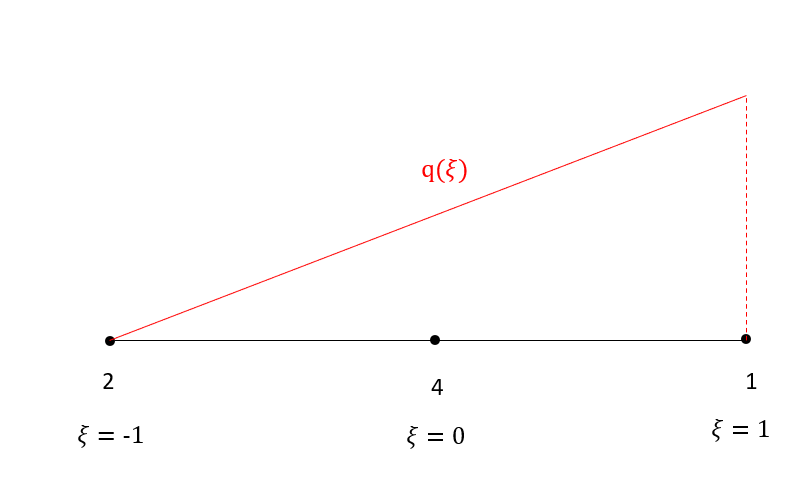
\includegraphics[width=0.6\textwidth,center]{fig/q1_prova_2012.PNG}
	\caption{Sistema de coordenadas da barra} 
	\label{provas:Lado do triangulo}
\end{figure}
%
Sendo assim,
%
\begin{equation}
	\begin{split}
	&N_2 = \frac{1}{2} \xi (\xi - 1) \\ 
	&N_4 = (1 + \xi) (1 - \xi) \\ 
	&N_1 = \frac{1}{2} \xi (1 + \xi)\\
	&q_x = \frac{q}{2} (1 + \xi)
	\end{split}  
\end{equation}
%
As integrais são,
\begin{equation}
	\begin{split}
		&f_2^x = \int_{\Gamma} N_2 q_x d\Gamma = \int_{-1}^{1} N_2 q_x det J d\xi = \frac{q L}{8} \int_{-1}^{1} \xi (\xi - 1) (1 + \xi) d\xi = 0\\
		&f_4^x = \int_{\Gamma} N_4 q_x d\Gamma = \int_{-1}^{1} N_4 q_x det J d\xi = \frac{q L}{4} \int_{-1}^{1} (1 + \xi)^2 (1 - \xi) d\xi =  \frac{q L}{3}\\
		&f_1^x = \int_{\Gamma} N_1 q_x d\Gamma = \int_{-1}^{1} N_1 q_x det J d\xi = \frac{q L}{8} \int_{-1}^{1} \xi (1 + \xi) (1 + \xi)  d\xi =  \frac{q L}{6}
	\end{split}
\end{equation}
%
 \begin{itemize}
	\item Usando as funções de interpolação do triangulo
\end{itemize}
%
Na Figura \ref{provas:coordenadas_de_area} temos as áreas utilizadas no sistema de coordenadas locais do triangulo. 
\begin{figure}[H]
	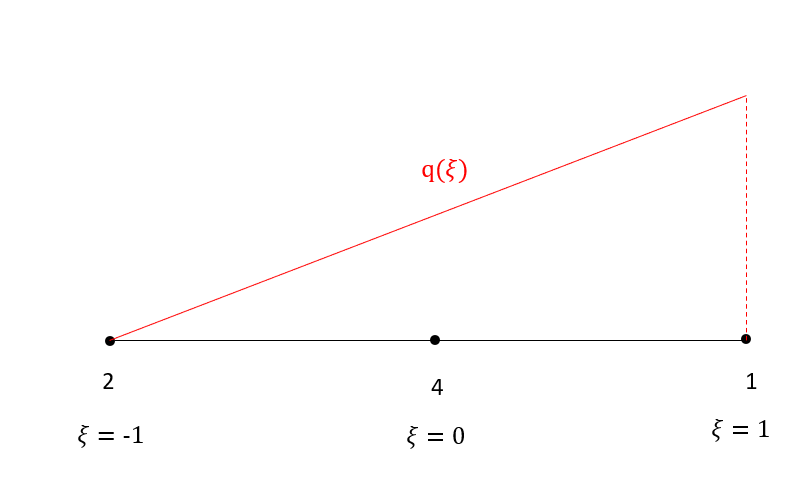
\includegraphics[width=0.6\textwidth,center]{fig/q1_prova_2012.PNG}
	\caption{Coordenadas de área do triângulo} 
	\label{provas:coordenadas_de_area}
\end{figure}
%
Se o ponto $P$ só pode estar na aresta 1-2. Nos temos que
%
\begin{equation}
	\begin{split}
		&\xi_1 = \frac{A_{31}}{A} = \frac{A_{31}}{A}\\
    	&\xi_2 = \frac{A_{23}}{A} = \frac{A - A_{31}}{A} = 1 -  \frac{A_{31}}{A} = 1 - \xi_1\\
		&\xi_3 = \frac{A_{12}}{A} = 0
	\end{split}
\end{equation} 
%
A funções de interpolação são
%
\begin{equation}
	\begin{split}
		&N_1 = \xi_1 (2 \xi_1 - 1) \\ 
		&N_4 = 4 \xi_1 \xi_2 = 4 \xi_1 (1 - \xi_1)\\ 
		&N_2 = \xi_2 (2 \xi_2 - 1) = (1 - \xi_1) (1 - 2 \xi_1)\\
		&q_x = q \xi_1
	\end{split}  
\end{equation}
%
As integrais são,
\begin{equation}
	\begin{split}
		&f_2^x = \int_{\Gamma} N_2 q_x d\Gamma = \int_{0}^{1} N_2 q_x det J d\xi = q L \int_{0}^{1} (1 - \xi_1) (1 - 2 \xi_1) \xi_1 d\xi = 0\\
		&f_4^x = \int_{\Gamma} N_4 q_x d\Gamma = \int_{0}^{1} N_4 q_x det J d\xi = 4 q L \int_{0}^{1} \xi_1 (1 - \xi_1) \xi_1 d\xi =  \frac{q L}{3}\\
		&f_1^x = \int_{\Gamma} N_1 q_x d\Gamma = \int_{0}^{1} N_1 q_x det J d\xi = q L \int_{0}^{1} \xi_1 (2\xi_1 - 1) \xi_1  d\xi =  \frac{q L}{6}
	\end{split}
\end{equation}
%
\color{blue}
Reposta:
\begin{equation}
	\begin{split}
		&\mathbf{f}_2
		= 
		\begin{bmatrix}
			0\\
			0
		\end{bmatrix}\\
		&\mathbf{f}_4
		= 
		\begin{bmatrix}
			\frac{q L}{3}\\
			0
		\end{bmatrix}\\
		&\mathbf{f}_1
		= 
		\begin{bmatrix}
		\frac{q L}{6}\\
		0
	\end{bmatrix}\\	
	\end{split}
\end{equation} 
\color{black}
%
A força resultante da aresta é $\frac{q L}{2}$. Para verificar a resposta vamos somar $f_1^x$, $f_2^x$ e $f_4^x$ para calcular a força resultante na aresta através das forças equivalentes nodai,
%
\begin{equation}
	f_r^x = f_1^x + f_2^x + f_4^x = \frac{q L}{6} + \frac{q L}{3} + 0 = \frac{q L}{2}
\end{equation}


\subsection{Q2 - prova - 2012}

Utilizando o meto do resíduos ponderados temos,
%
\begin{equation}
	\int_{\Omega} \left[k \left(\mdpv{\phi}{x} + \mdpv{\phi}{y}\right) + Q\right]w d\Omega = 0	
\end{equation}
%
Expandindo as integral temos,
%
\begin{equation}
	\int_{\Omega} k \mdpv{\phi}{x} w d\Omega + \int_{\Omega} k \mdpv{\phi}{y} w d\Omega + \int_{\Omega} Q w d\Omega = 0
	\label{provas:passo_intermediario}
\end{equation}
%
O objetivo agora é diminuir a ordem da deriva de $\phi$, nós queremos apenas derivadas primeira em $\phi$. Pelo teorema do divergente temos,
%
\begin{equation}
	\begin{split}
	&\int_{\Omega} \mdp{} {x} \left( k \mdp{\phi}{x} w \right) d\Omega = \int_{\Gamma} \left(k \mdp{\phi}{x}\right) w n_x d\Gamma\\
	&\int_{\Omega} \mdp{} {y} \left( k \mdp{\phi}{y} w \right) d\Omega = \int_{\Gamma} \left(k \mdp{\phi}{y}\right) w n_y d\Gamma
    \end{split}
	\label{provas:gauss}
\end{equation}
%
Pela integra por partes temos,
%
\begin{equation}
	\begin{split}
	&\int_{\Omega} \mdp{} {x} \left( k \mdp{\phi}{x} w \right) d\Omega = \int_{\Omega} k \mdpv{\phi}{x} w d\Omega + \int_{\Omega} k \mdp{\phi}{x} \mdp{w} {x}  d\Omega\\
	&\int_{\Omega} \mdp{} {y} \left( k \mdp{\phi}{y} w \right) d\Omega = \int_{\Omega} k \mdpv{\phi}{y} w d\Omega + \int_{\Omega} k \mdp{\phi}{y} \mdp{w} {y}  d\Omega\\
	\end{split}
	\label{provas:partes}
\end{equation}
%
Juntando a eq. (\ref{provas:gauss}) e eq. (\ref{provas:partes}),
%
\begin{equation}
	\begin{split}
		&\int_{\Gamma} \left(k \mdp{\phi}{x}\right) w n_x d\Gamma = \int_{\Omega} k \mdpv{\phi}{x} w d\Omega + \int_{\Omega} k \mdp{\phi}{x} \mdp{w} {x}  d\Omega\\
		&\int_{\Gamma} \left(k \mdp{\phi}{y}\right) w n_y d\Gamma = \int_{\Omega} k \mdpv{\phi}{y} w d\Omega + \int_{\Omega} k \mdp{\phi}{y} \mdp{w} {y}  d\Omega\\
	\end{split}
\end{equation}
%
Rearranjando os termos,
%
\begin{equation}
	\begin{split}
		&\int_{\Omega} k \mdpv{\phi}{x} w d\Omega = \int_{\Gamma} \left(k \mdp{\phi}{x}\right) w n_x d\Gamma - \int_{\Omega} k \mdp{\phi}{x} \mdp{w} {x} d\Omega\\
		&\int_{\Omega} k \mdpv{\phi}{y} w d\Omega = \int_{\Gamma} \left(k \mdp{\phi}{y}\right) w n_y d\Gamma - \int_{\Omega} k \mdp{\phi}{y} \mdp{w} {y} d\Omega\\
	\end{split}
	\label{provas:divergente+partes}
\end{equation}
%
Agora com a eq. (\ref{provas:divergente+partes}) podemos voltar para a eq. (\ref{provas:passo_intermediario})
%
\begin{equation}
	\begin{aligned}
	&\int_{\Gamma} \left(k \mdp{\phi}{x}\right) w n_x d\Gamma + \int_{\Gamma} \left(k \mdp{\phi}{y}\right) w n_y d\Gamma - \int_{\Omega} k \mdp{\phi}{y}\mdp{w}{y} d\Omega\\
	& - \int_{\Omega} k \mdp{\phi}{x} \mdp{w}{x} d\Omega + \int_{\Omega} Q w d\Omega = 0 
	\end{aligned}
\end{equation}
%
Rearranjando os termos,
%
\begin{equation}
\int_{\Omega} k \left(\mdp{\phi}{x} \mdp{w}{x} + \mdp{\phi}{y} \mdp{w}{y} \right) d\Omega = \int_{\Gamma} k \left(\mdp{\phi}{x} n_x + \mdp{\phi}{y} n_y \right) w d\Gamma + \int_{\Omega} Q w d\Omega 
\end{equation}
%
Considerando agora a condição de contorno natural,
%
\begin{equation}
	q = k \mdp{\phi}{n} = k \left(\mdp{\phi}{x} n_x + \mdp{\phi}{y} n_y\right)
\end{equation}
%
A formulação variacional final é (pag. 168),

\color{blue}
Reposta a):
\begin{equation}
	\int_{\Omega} k \left(\mdp{\phi}{x} \mdp{w}{x} + \mdp{\phi}{y} \mdp{w}{y} \right) d\Omega = \int_{\Gamma_2} q w d\Gamma + \int_{\Omega} Q w d\Omega 
\end{equation}
\color{black}
%
%
\begin{itemize}
	\item Questão b)
\end{itemize}
%
Definindo as aproximações para $\phi$ e $w$,
% 
\begin{equation}
	\begin{split}
		&\phi = \sum_{j=0}^n N_j \phi_j\\
		&w = \sum_{i=0}^n N_i w_i
	\end{split}
\end{equation}
%
Substituindo na resposta a) chega-se à:

\color{blue}
Reposta b):
\begin{equation}
	\begin{split}
		&k_{ij} = \int_{\Omega} k \left( \mdp{N_j}{x}\mdp{N_i}{x} + \mdp{N_j}{y}\mdp{N_i}{y} \right) d \Omega\\
		&f_{i} = \int_{\Gamma_2} q N_i d\Gamma + \int_{\Omega} Q N_i d \Omega
	\end{split}
\end{equation}
\color{black}
%
\begin{itemize}
	\item Questão c)
\end{itemize}

Como as derivada que aparecem na integral de omega são de primeira ordem temos que as funções aproximação precisam ser da classe $C^0$ pela condição de compatibilidade. Isso implica que as aproximação que ser no mínimo linear. A outra condição é de completidade, as aproximações tem que ser um polinômio completo. Ou seja tem que ser da forma:

\begin{equation}
A_p x^p + A_{p-1} x^{p-1} + A_{p-2}x^{p-2} ... + A_1 x + A_0 x^0
\end{equation}



\subsection{Q3 - prova - 2012}

A área do retângulo pode ser escrita na forma de uma integral. Além disso o determinante da jacobiano de uma paralelogramo é constante, assim temos,
%
\begin{equation}
	\begin{split}
		&A = \int_A dA = \int_{-1}^{1} \int_{-1}^{1} det J d\eta d\xi\\
		&A = det J \int_{-1}^{1} \int_{-1}^{1} d\eta d\xi\\
		&A = det J 4
	\end{split}
\end{equation}
%
\color{blue}
Reposta:
\begin{equation}
	det J = \frac{A}{4}
\end{equation} 
\color{black}

\section{Integral nos elementos}

\begin{equation}
k_{45} = \int_{\Omega} \mdp{N_5}{x}\mdp{N_4}{x} + \mdp{N_5}{y}\mdp{N_4}{y} d \Omega
\end{equation}
%
Para coordenadas locais do triangulo temos: 
%
\begin{equation}
k_{45} = k^e_{12} = \int_{0}^{1} \int_{0}^{1-\xi_1} \left( \mdp{N_2}{x}\mdp{N_1}{x} + \mdp{N_2}{y}\mdp{N_1}{y} \right) |J| d \xi_1 d \xi_2 
\end{equation}
%
A matriz jacobiana é:
%
\begin{equation}
	J = 
	\begin{bmatrix}
		\Delta x_{46} & \Delta y_{46}\\
		\Delta x_{56} & \Delta y_{56}\\
	\end{bmatrix}
\end{equation}
%
O determinante do jacobiano é:
%
\begin{equation}
	|J| = 2A
\end{equation}
%
As derivadão são calcular pela a inversa do jacobiano,
%
\begin{equation}
	\begin{bmatrix}
	\mdp{N_i}{x}\\
	\mdp{N_i}{y}\\
	\end{bmatrix}	
	=
	\frac{1}{|J|}
	\begin{bmatrix}
	\Delta y_{56}&-\Delta y_{46}\\
	-\Delta x_{56}&\Delta x_{46}\\
	\end{bmatrix}
	\begin{bmatrix}
	\mdp{N_i}{\xi_1}\\
	\mdp{N_i}{\xi_2}\\
\end{bmatrix}
\end{equation}
%
As derivadas são,
%
\begin{equation}
\begin{split}
	&\mdp{N_1}{x} =  \frac{\Delta y_{56}}{|J|}\\
	&\mdp{N_1}{y} = -\frac{\Delta x_{56}}{|J|} = \frac{\Delta x_{65}}{|J|}\\
	&\mdp{N_2}{x} = -\frac{\Delta y_{46}}{|J|} = \frac{\Delta y_{64}}{|J|}\\
	&\mdp{N_2}{y} =  \frac{\Delta x_{46}}{|J|}\\		
\end{split}
\end{equation}
%
Substituindo na integral,
%
\begin{equation}
\begin{split}
	&k^e_{12} = \int_{0}^{1} \int_{0}^{1-\xi_1} \left(\frac{\Delta y_{64}}{|J|} \frac{\Delta y_{56}}{|J|} + \frac{\Delta x_{46}}{|J|} \frac{\Delta x_{65}}{|J|} \right) |J| d \xi_1 d \xi_2\\
	& k^e_{12} = \left(\frac{\Delta y_{64}}{|J|} \frac{\Delta y_{56}}{|J|} + \frac{\Delta x_{46}}{|J|} \frac{\Delta x_{65}}{|J|} \right) |J| \int_{0}^{1} \int_{0}^{1-\xi_1} d \xi_1 d \xi_2\\
	& k^e_{12} = \frac{\Delta y_{64} \Delta y_{56} + \Delta x_{46} \Delta x_{65}}{4 A}
\end{split}
\end{equation}
%



%---------------------------------------------------------------------------

\end{document}
%---------------------------------------------------------------------------
